\chapter{Estado del arte}
\label{ch:estado}

\section{Realidad aumentada}
 Una de las primeras definiciones de realidad aumentada fue dada por Ronald Azuma en 1997 \cite{azuma}, y dice que la Realidad Aumentada es cualquier sistema que combine elementos reales y virtuales, que sea interactivo en tiempo real y que sea registrado en tres dimensiones. Por tanto, la realidad aumentada es una tecnología que permite añadir información virtual al mundo real a través de un dispositivo, es decir, permite mostrar el mundo real con objetos virtuales en éste, por lo que no pretende crear un mundo virtual, sino complementar al mundo real con más información.

\section{Diferencias entre realidad aumentada, realidad virtual y realidad mixta}
Realidad virtual: Es una tecnología completamente inmersiva que consiste en convencer a tus sentidos de que estas en otro mundo que no es el real, es un mundo virtual. Usando un dispositivo que se coloca en la cabeza, la realidad virtual permite disfrutar de un mundo de imágenes y sonidos generado por ordenador en el que puedes manipular objetos, y moverte por dicho mundo usando controladores hápticos conectados a un ordenador o a una consola. \cite{intel}

Realidad aumentada: Es una tecnología que superpone información digital sobre elementos del mundo real. El elemento central es el mundo real, pero lo mejora con otros detalles digitales, complementando así la realidad. \cite{intel}

Realidad mixta: Es una tecnología que hace converger el mundo real y elementos digitales. En esta puedes interactuar y manipular tanto elementos físicos como virtuales. La realidad mixta te permite sumergirte en el mundo que te rodea incluso cuando tú interactúas con el entorno virtual usando tus propias manos. Esta tecnología te permite tener un pie en el mundo real y el otro en un lugar imaginario. \cite{intel}

\section{Aplicaciones de la realidad aumentada}
\begin{itemize}
  \item Medicina: La realidad aumentada puede aportar grandes avances a la medicina, ya que permite la visualización en 3D de objetos que bien pueden ser órganos o partes del cuerpo en el mundo real, por lo que puede facilitar a los doctores muchas tareas que requieran el estudio de modelos 3D. Por ejemplo, los doctores pueden utilizar la realidad aumentada con el objetivo de prepararse para una operación como se puede observar en la Figura \ref{figura-medicina}, o simplemente para tareas de visualización médica, de igual manera que actualmente se utilizan los TAC o las resonancias magnéticas, pero los datos obtenidos con dichos escáneres se convertirían en modelos 3D que son mucho más sencillos de explorar que un conjunto de imágenes 2D. También se podría utilizar la realidad aumentada con el objetivo de entrenamiento para cirujanos que se están formando, mostrándoles instrucciones sobre un modelo 3D de cómo se debería realizar una determinada operación, ayudando así a que no necesiten consultar un manual y quitar la vista del “paciente” si no que todo sería sobre dicho “paciente” que realmente es un modelo 3D. \cite{azuma}

  \begin{figure}[h]
    \centering
    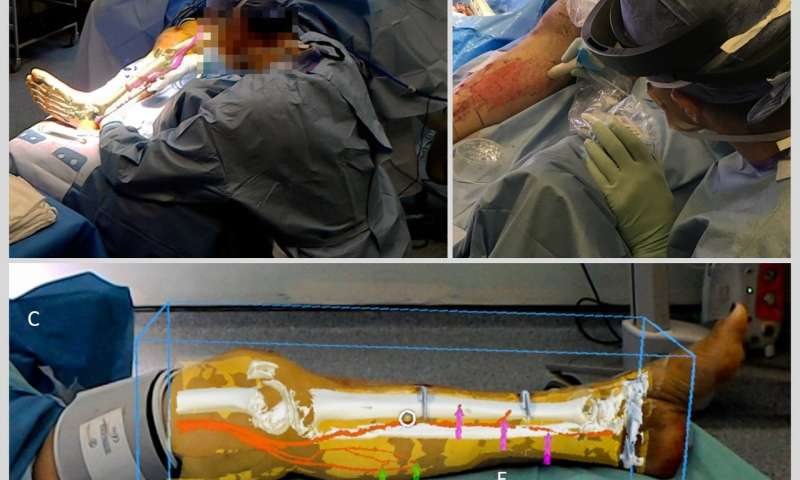
\includegraphics[scale=0.5]{medicine}
    \caption{Profesionales médicos utilziando realidad aumentada como ayuda para una operación.\protect\footnotemark}
    \label{figura-medicina}
  \end{figure}

  \footnotetext{ Philip Pratt, et al. Eur Radiol Exp, 2018}

  \newpage

  \item Educación: La realidad aumentada tiene mucho que aportar a la educación, ya que permite una forma interactiva de aprender que los libros no permiten. Por ejemplo, que mejor manera de aprender el sistema respiratorio que con uno a tamaño real en 3D que tu puedes explorar. Y la realidad aumentada no implica que los libros no sirvan y vayan a desaparecer, si no que puede suponer un complemento para dichos libros como se puede observar en la Figura \ref{figura-educacion}, cambiando la forma en la que nos relacionamos con ellos, por ejemplo, con imágenes en los libros que al escanearlas muestren elementos 3D que nos permitan comprender mejor el contenido que se está exponiendo en dicho libro. \cite{reinoso}

  \begin{figure}[h]
    \centering
    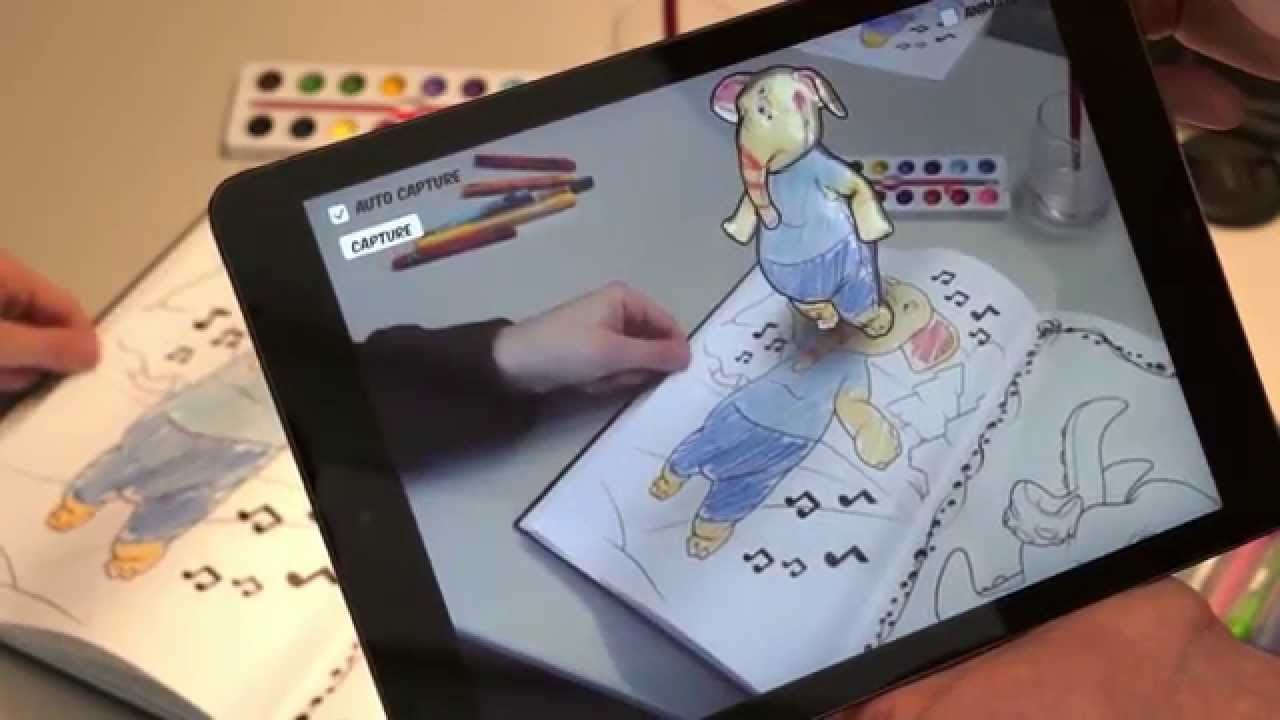
\includegraphics[scale=0.2]{education}
    \caption{Libro que utiliza la realidad aumentada para mostrar el dibujo en 3D.\protect\footnotemark}
    \label{figura-educacion}
  \end{figure}

  \footnotetext{ \url{https://www.youtube.com/watch?v=IeHKVC0XLe4}, Alibabach}

  \begin{figure}[h]
    \centering
    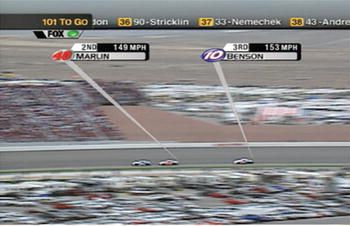
\includegraphics[scale=0.7]{entertainment1}
    \caption{Imagen que muestra la utilización de realidad aumentada en la retransmisión de deportes. \cite{van-krevelen}}
    \label{figura-entretenimiento1}
  \end{figure}

  \item Entretenimiento: La realidad aumentada se puede aplicar en el entretenimiento relacionada a juegos, por ejemplo, mostrando los tableros de juego en una superficie plana en lugar de en la pantalla en 2D, como se puede ver en la Figura \ref{figura-entretenimiento}, pero también se puede aplicar la realidad aumentada en otras formas de entretenimiento diferentes, por ejemplo, en los deportes que se retransmiten, mostrando información relevante para los usuarios sobre dicho deporte, por ejemplo, en las carreras de coches, ya que puede estar grabado desde cierta distancia mostrar sobre cada coche información de quien es, su puesto y la velocidad que lleva como se puede ver en la Figura \ref{figura-entretenimiento1}. \cite{van-krevelen}

  \begin{figure}[h]
    \centering
    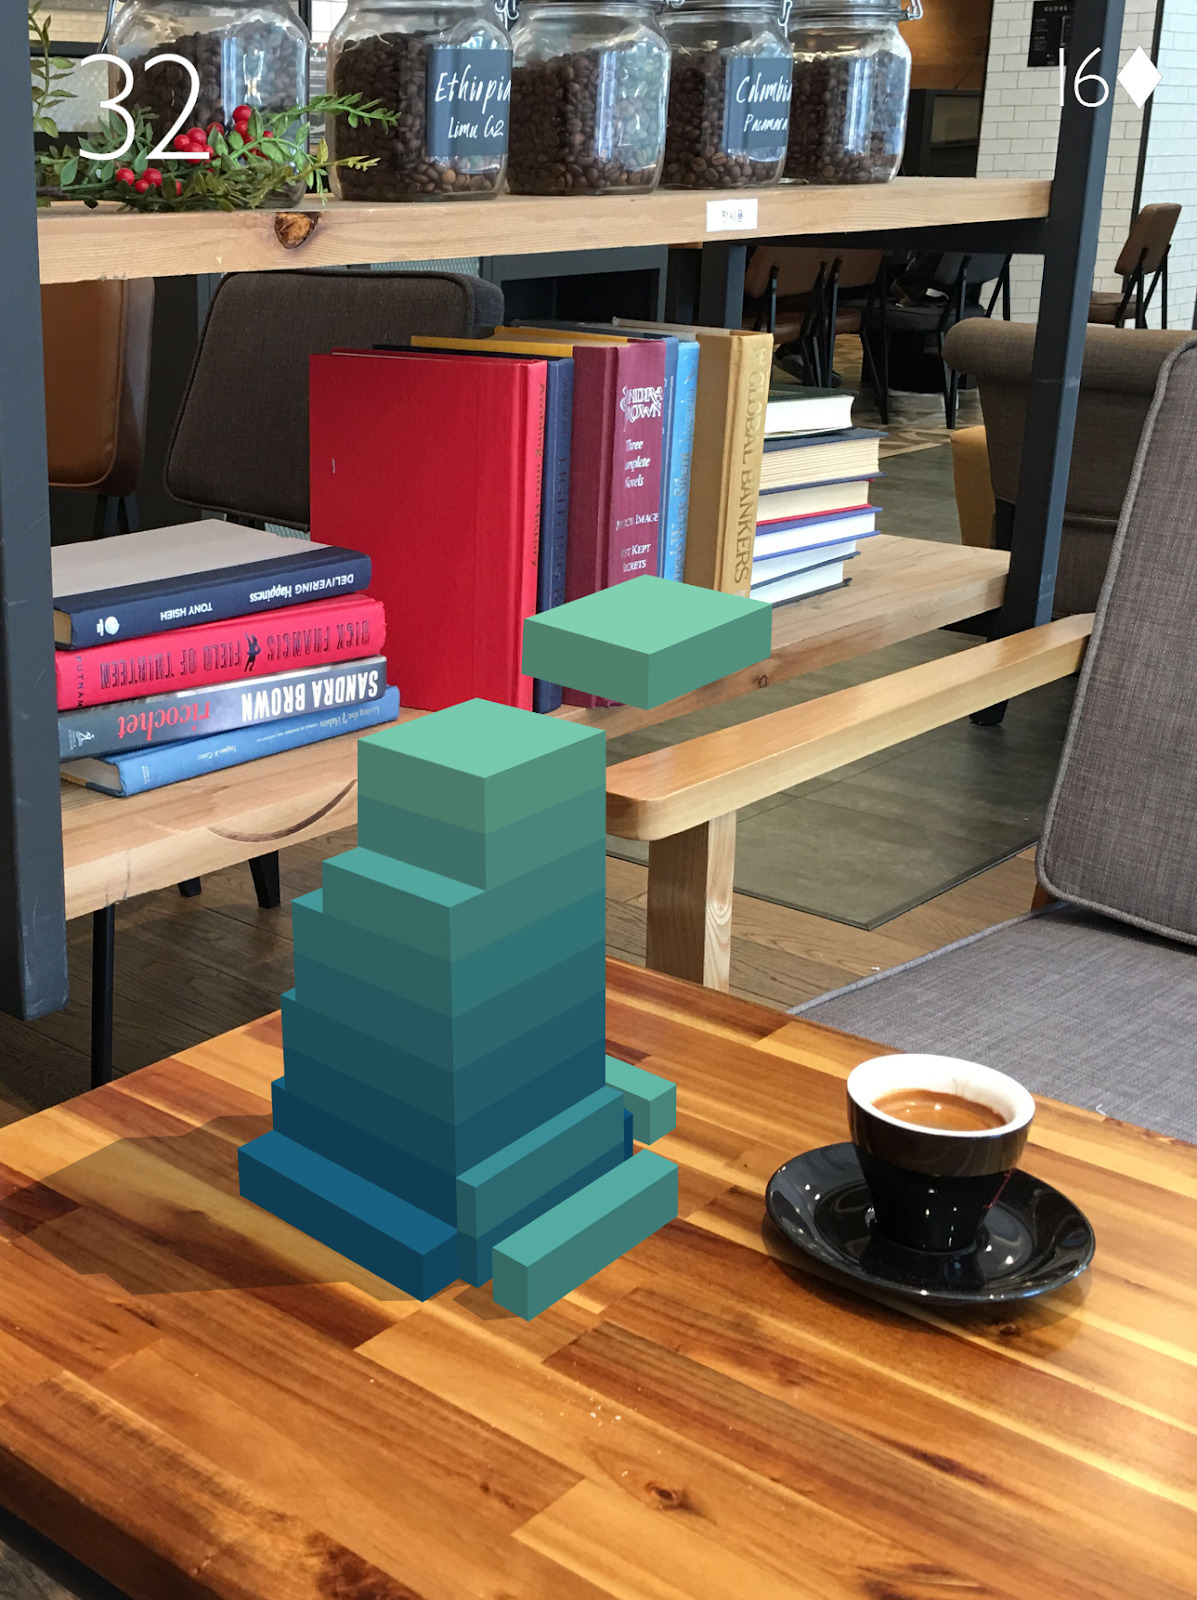
\includegraphics[scale=0.1]{entertainment}
    \caption{Imagen que muestra la utilización de realidad aumentada en un juego.\protect\footnotemark}
    \label{figura-entretenimiento}
  \end{figure}

  \footnotetext{ \url{https://itunes.apple.com/us/app/stack-ar/id1269638287?mt=8}, Ketchapp}

  \item Turismo: La realidad aumentada puede dar una vuelta al turismo, teniendo un guia turistico en tu propio dispositivo móvil, por ejemplo, mediante el uso de realidad aumentada que utiliza la geolocalización, puede indicar los monumentos relevantes de la ciudad, la distancia a ellos y donde están a través de la cámara de un dispositivo móvil. También puede mejorar las experiencias turísticas actuales de una forma mucho más visual, cuando se esté en un sitio histórico te puede contar la historia de una forma más entretenida y visual, mostrando elementos 3D en el lugar, recreando lo que sucedió, como se puede observar en la Figura \ref{figura-turismo}. \cite{reinoso}

  \begin{figure}[h]
    \centering
    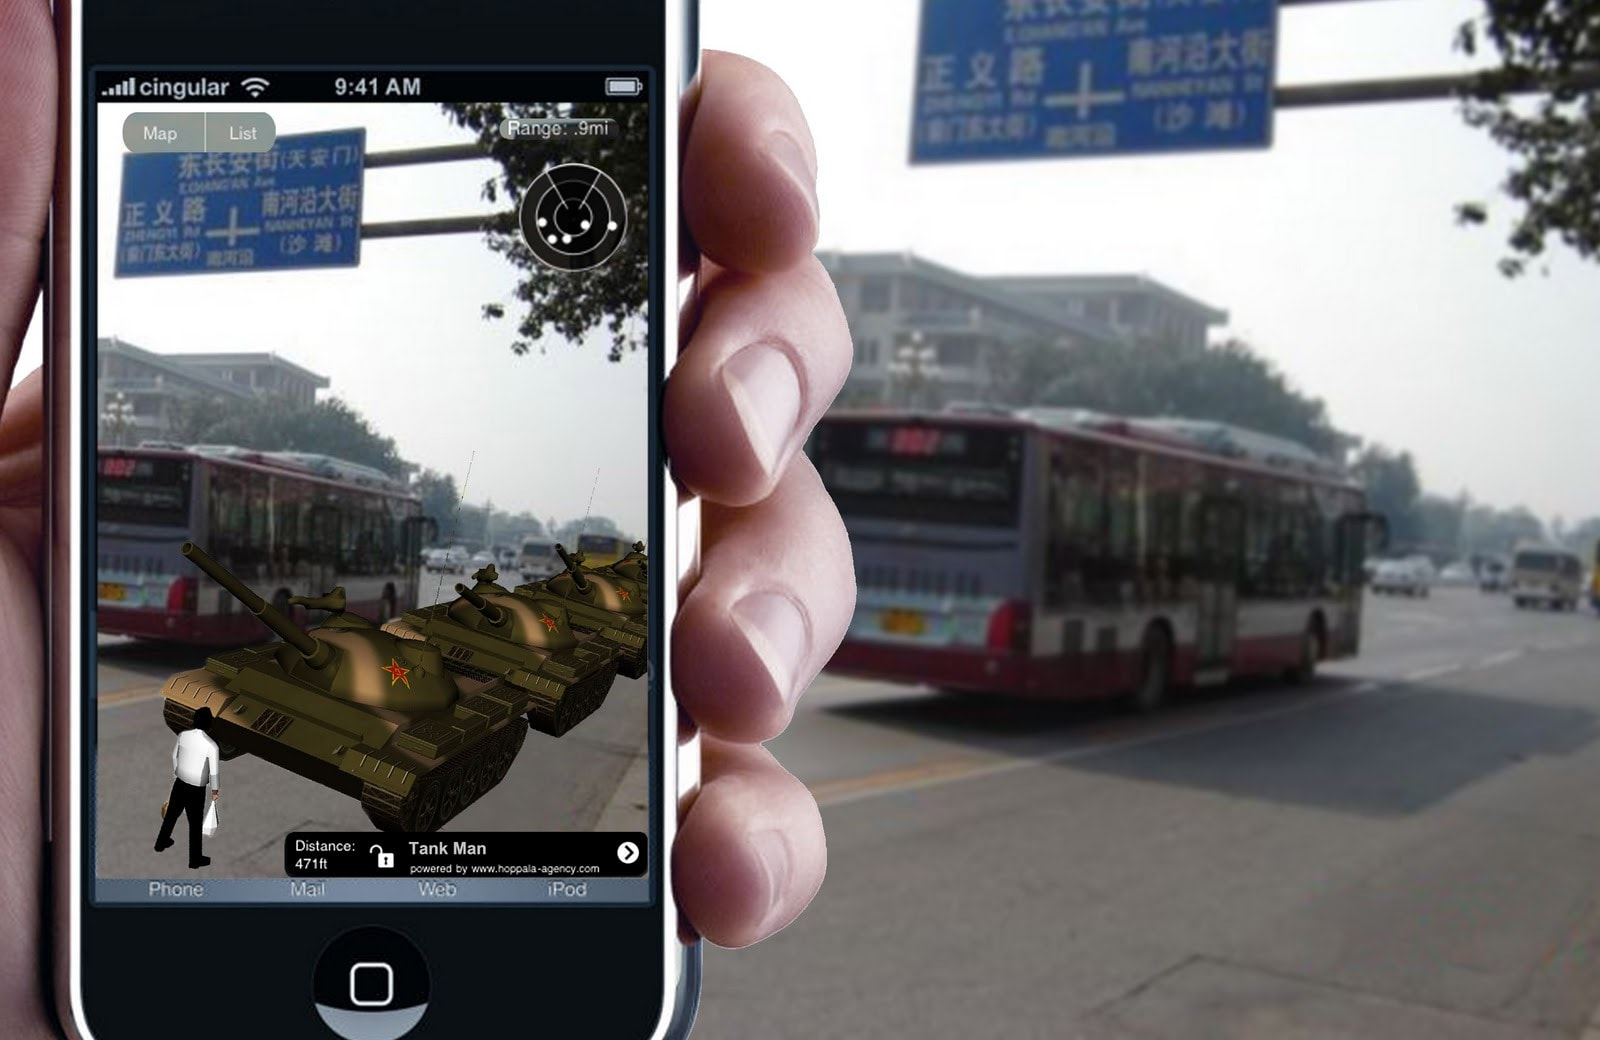
\includegraphics[scale=0.15]{turism}
    \caption{Imagen que muestra un hecho historico visualizandose con realidad aumentada. \cite{layar}}
    \label{figura-turismo}
  \end{figure}

  \newpage

  \item Comercio: La realidad aumentada puede revolucionar el sector de las ventas por internet, la mayor desventaja actual que tiene comprar por internet es que el usuario se tiene que conformar con imágenes 2D del producto, la realidad aumentada permite romper esa barrera, y mostrar al usuario el producto en 3D, en tamaño real en su propia casa, por ejemplo, esto es muy útil con muebles ya que necesitas las medidas del hueco que tienes y del mueble para saber si encajará en el hueco o simplemente si queda bonito en la habitación, con la realidad aumentada ambos problemas están solucionados, puedes ver el mueble en el hueco que quieres en tamaño real, lo que te permite saber si cabe y si queda bien. Un ejemplo de este tipo de aplicación se puede observar en la Figura \ref{figura-comercio}.

  \begin{figure}
    \centering
    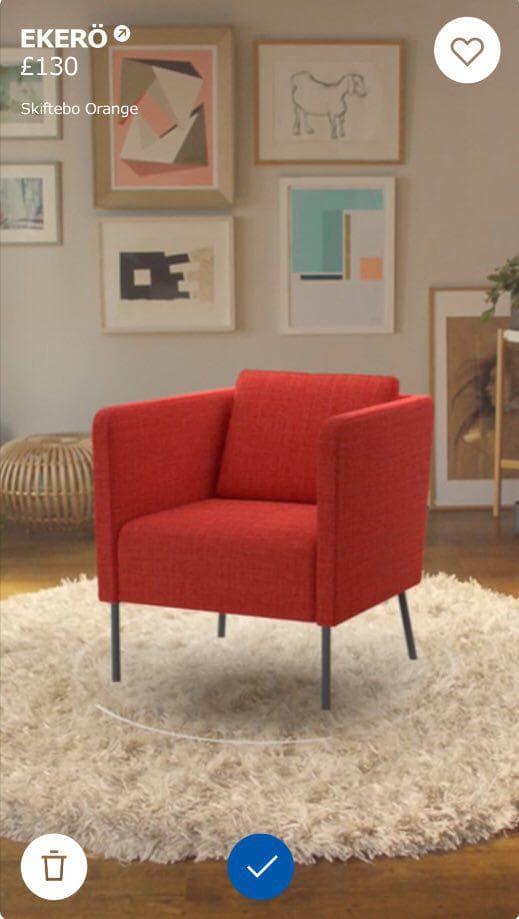
\includegraphics[scale=0.3]{commerce}
    \caption{Imagen que muestra la utilización de realidad aumentada en un juego.\protect\footnotemark}
    \label{figura-comercio}
  \end{figure}

  \footnotetext{ \url{https://itunes.apple.com/es/app/ikea-place/id1279244498?mt=8}, Ikea}

\end{itemize}

\newpage

\section{Formas de integrar la información digital con el mundo real \cite{prendes-espinosa}}

\begin{itemize}
  \item Vincular la información a un marcador: Un marcador es una imagen en blanco y negro que contiene un patrón, como puede ser un código QR, un ejemplo de marcador se puede ver en la Figura \ref{figura-marcador}. Este tipo de tecnologóia almacena en memoria marcadores, y cuando se escanea dicho marcador se puede mostrar una información asociada a este con respecto a la posición de dicho marcador, como se puede ver en la Figura \ref{figura-marcador-aumentado}.

  \begin{figure}
    \centering
    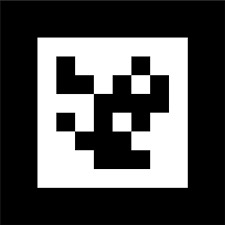
\includegraphics[scale=0.3]{marker}
    \caption{Imagen que muestra un ejemplo de marcador.}
    \label{figura-marcador}
  \end{figure}

  \begin{figure}[h]
    \centering
    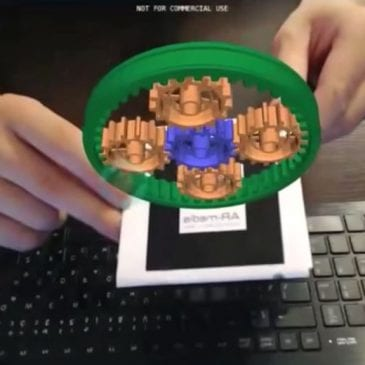
\includegraphics[scale=0.5]{marker-augmented}
    \caption{Imagen que muestra un marcador con un modelo 3D asociado a este.}
    \label{figura-marcador-aumentado}
  \end{figure}

  \newpage

  \item Vincular la información a una imagen fija o móvil: Lo que hace es almacenar en memoria imágenes, y cuando dichas imágenes se escanean se puede mostrar una información asociada a dicha imagen con respecto a la posición de la imagen, cabe la posibilidad de que cuando dicha imagen esté en movimiento se pierda la información asociada a esta y se muestre cuando vuelva a estar fija, o por el contrario que dicha información asociada se desplace junto con la imagen. Podemos observar un ejemplo en la Figura \ref{figura-image}.

  \begin{figure}[h]
    \centering
    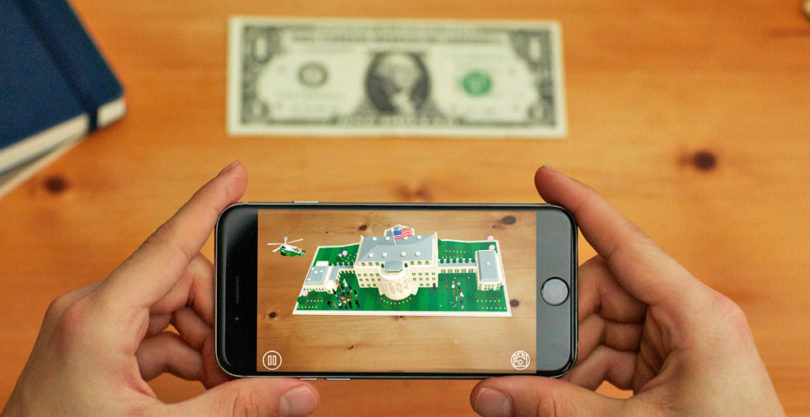
\includegraphics[scale=0.3]{image}
    \caption{Imagen que muestra una imagen con un modelo 3D asociado a esta.\protect\footnotemark}
    \label{figura-image}
  \end{figure}

  \footnotetext{ \url{https://vrscout.com/news/augmented-reality-app-1-dollar-bill-tour-white-house/}, Kyle Melnick}

  \newpage

  \item Vincular la información a un objeto 3D: Lo que ocurre es que se tendrá almacenado en memoria un modelo del objeto, y con dispositivos como Kinect (mostrado en la Figura \ref{figura-kinect}) se puede reconocer dicho objeto y asociar una información a este.

  \begin{figure}[h]
    \centering
    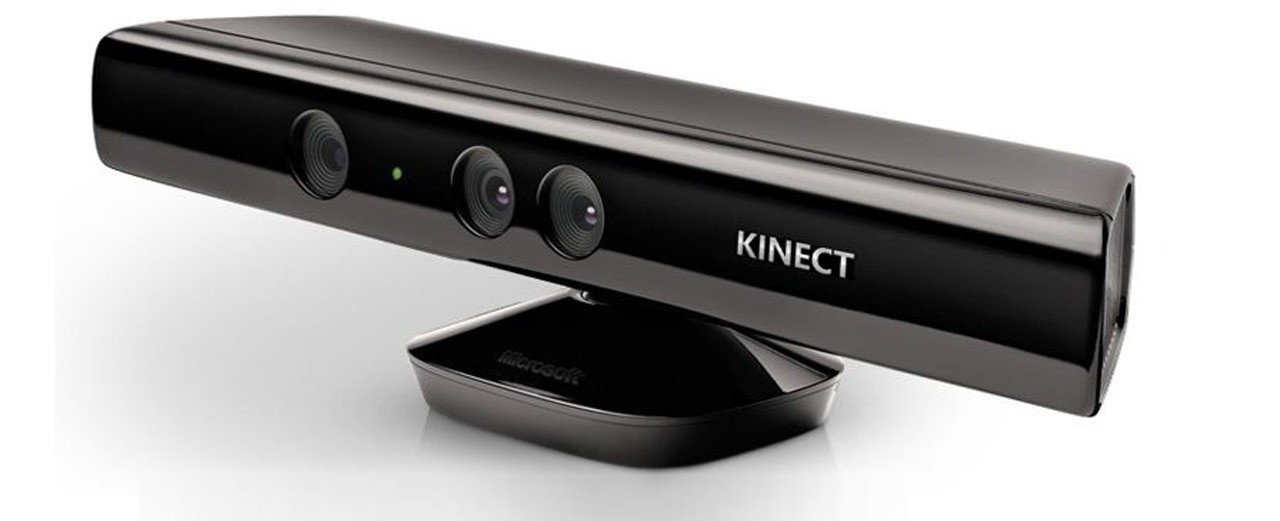
\includegraphics[scale=0.2]{kinect}
    \caption{Imagen que muestra la herramienta kinect.}
    \label{figura-kinect}
  \end{figure}

  \item Vincular la información a una escena:  Lo que hace esta técnica es escanear el mundo real y asignar coordenadas, escaneará las superficies planas horizontales y verticales, y establecerá un modelo 3D de estas, en el que establece coordenadas, y a cada una de estas coordenadas se puede asociar información con respecto a la posición de esta, como se puede ver en la Figura \ref{figura-scene}, lo que nos permitirá gracias a que se escanea el mundo en 3D que al movernos alrededor, incluso si dejamos de tener la coordenada dentro de la visión de la cámara, que al volver a mirar al punto de la coordenada la información asociada siga ahí.

  \begin{figure}[h]
    \centering
    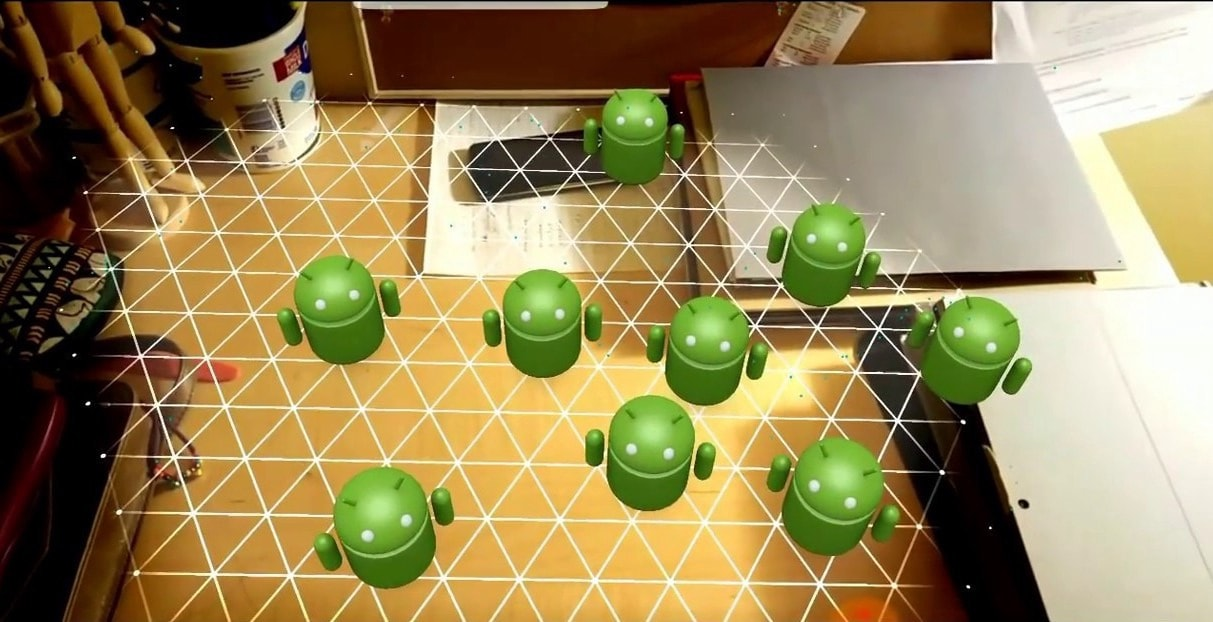
\includegraphics[scale=0.3]{scene}
    \caption{Imagen que muestra el reconocimiento de superficies de una escena y la asociación de información a una coordenada de esta escena.}
    \label{figura-scene}
  \end{figure}

  \item Vincular la información a una coordenada del mundo real: Se tendrá la información asignada a dicha coordenada del mundo, y gracias al sistema gps del dispositivo y otros sensores, permite que cuando dicha coordenada entre en el rango de visión del dispositivo, muestre la información asociada a esta, como se puede observar en la Figura \ref{figura-location}.

  \begin{figure}[h]
    \centering
    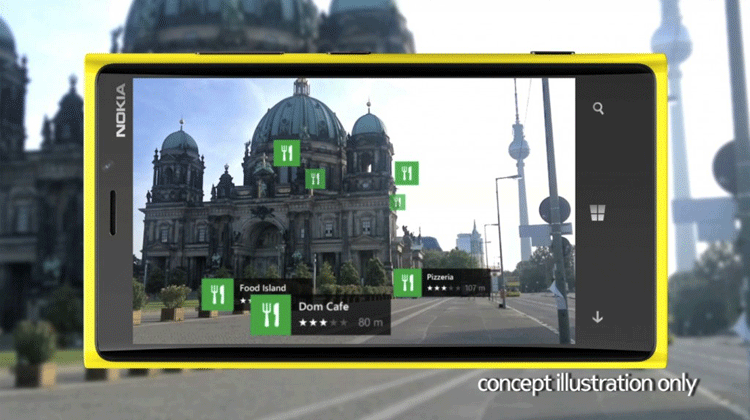
\includegraphics[scale=0.3]{location}
    \caption{Imagen que muestra la visualización de información asociada a coordenadas del mundo real.\protect\footnotemark}
    \label{figura-location}
  \end{figure}

  \footnotetext{ \url{https://www.gislounge.com/augmented-reality-digital-map-revolution/}, Nokia}

\end{itemize}

\section{Dispositivos y técnicas de visualización \cite{billinghurst}}
Existen diferentes tipos de pantallas para la visualización de realidad aumentada:
\begin{itemize}
  \item Pantallas basadas en video: Estas pantallas mediante procesos digitales combinan imágenes virtuales con video del mundo real. Estas pantallas son las más populares al estar en los dispositivos que usamos en el dia a dia como smartphones y tablets, como se puede ver en la Figura \ref{figura-pantalla-video}.

  \begin{figure}[h]
    \centering
    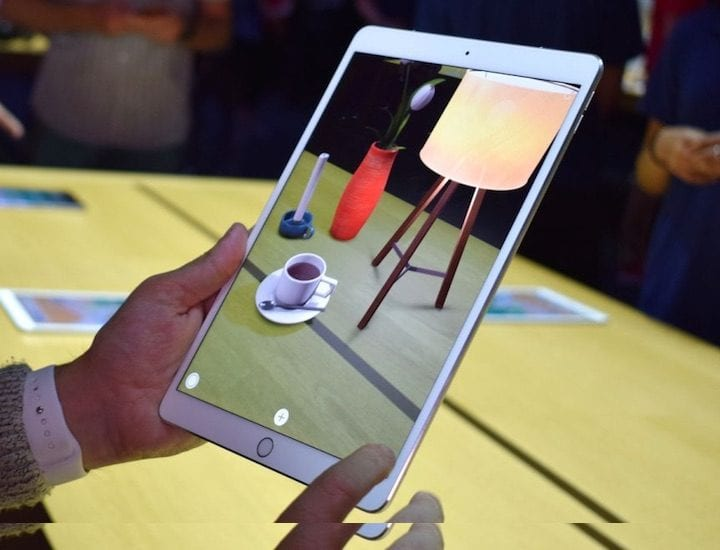
\includegraphics[scale=0.35]{video-screen}
    \caption{Imagen que muestra una tablet usando una aplicación de realidad aumentada.}
    \label{figura-pantalla-video}
  \end{figure}

  \newpage

  \item Pantallas ópticas transparentes: Estas pantallas mediante sistemas ópticos combinan imágenes virtuales con video del mundo real. Normalmente estas pantallas incluyen separadores de rayos, como un medio espejo, que permiten que en ese separador se vea la vista del mundo real a través del espejo, y los elementos virtuales añadidos, reflejados en el espejo, procedentes de una pantalla. En la Figura \ref{figura-pantalla-optica} se puede ver un esquema del funcionamiento de este tipo de pantallas.

  \begin{figure}[h]
    \centering
    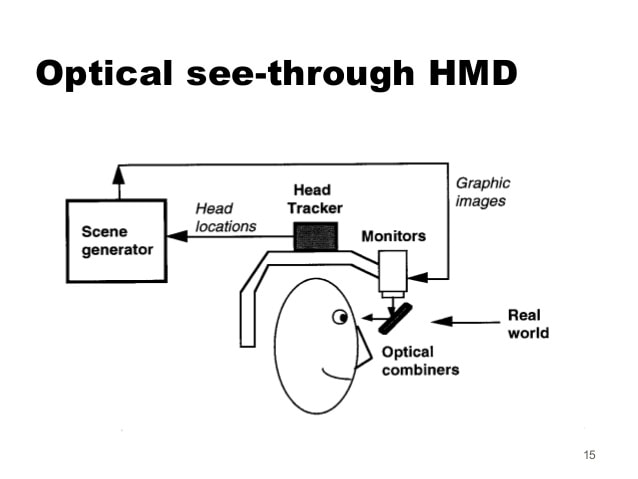
\includegraphics[scale=0.45]{optical-seethrough-screen}
    \caption{Imagen que muestra un esquema de como funcionan las pantallas opticas transparentes.}
    \label{figura-pantalla-optica}
  \end{figure}

  \newpage

  \item Pantallas basadas en proyección: Estas se encargan de proyectar las imágenes virtuales directamente sobre objetos del mundo real, como se puede ver en la Figura \ref{figura-pantalla-proyeccion}, esto combinado con el seguimiento de la posición del usuario y del objeto 3D, permite una aumentación interactiva. Por lo general, estos dispositivos suelen incluir un proyector montado en el techo o paredes.

  \begin{figure}[h]
    \centering
    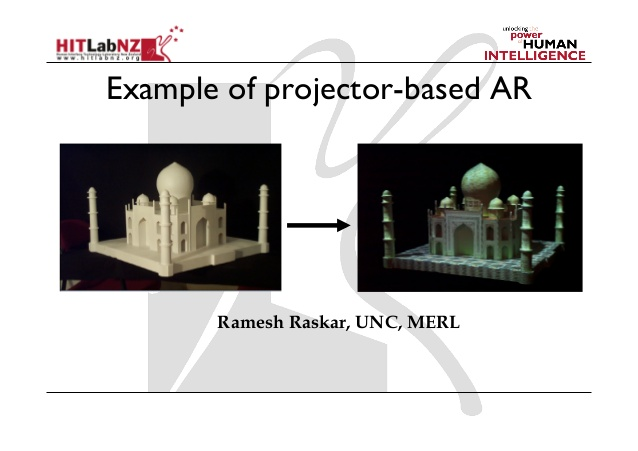
\includegraphics[scale=0.45]{projection-screen}
    \caption{Imagen que muestra como sobre un objeto se proyecta para conseguir una apariencia de objeto real.\protect\footnotemark}
    \label{figura-pantalla-proyeccion}
  \end{figure}

  \footnotetext{{\tt 2013 426 Lecture 2: Augmented Reality Technology. [Diapositivas de Power Point]. Recuperado de }\\
  \url{https://www.slideshare.net/marknb00/2013-426-lecture-2-augmented-reality-technology}. {\tt Billinghurst, M. (23 de julio de 2013).}}

  \item Pantallas de ojo multiplexado: Esta pantalla a diferencia de las anteriores no proporciona el mundo real con las imágenes virtuales ya mezcladas, si no que le proporciona al usuario ambas vistas y es el usuario el encargado de combinarlas mentalmente. Normalmente estas pantallas se suelen situar bastante cerca del ojo del usuario, para facilitar así la integración de los elementos virtuales que la pantalla muestra en el mundo real. Un ejemplo de visión con este tipo de pantallas se puede observar en la Figura \ref{figura-ojo-multiplexado}.

  \begin{figure}[h]
    \centering
    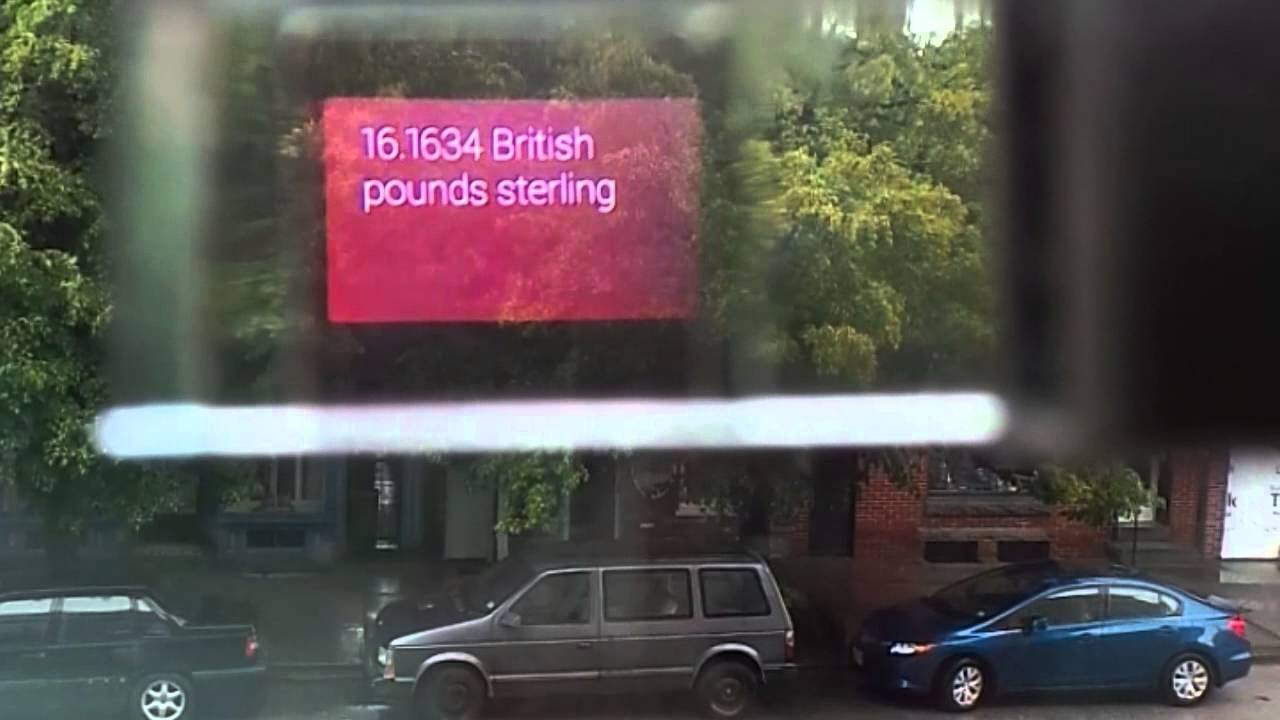
\includegraphics[scale=0.2]{multiplexed-eye}
    \caption{Imagen que muestra como es llevar las Google Glass puestas.\protect\footnotemark}
    \label{figura-ojo-multiplexado}
  \end{figure}

  \footnotetext{ \url{https://www.youtube.com/watch?v=d-y3bEjEVV8}, Phandroid}

\end{itemize}

\newpage

\begin{flushleft}
Otra forma de categorizar los tipos de pantalla puede ser la siguiente:
\end{flushleft}

\begin{itemize}
  \item Head-attached displays: Son dispositivos que van colocados en al cabeza del usuario, y que pueden ser desde el tamaño de un casco al tamaño de unas gafas.

  \item Hand-held display: Son dispositivos que el usuario puede sujetar con las manos, generalmente serán smartphones y tablets.

  \item Spatial displays: Suelen ser pantallas que están colocadas en un dispositivo o habitación, por lo que no permiten mucha movilidad.

\end{itemize}

\begin{flushleft}
Algunos ejemplos de Head-attached displays:
\end{flushleft}

\begin{itemize}
  \item Hololens: Este dispositivo entraría dentro de las pantallas ópticas transparentes, básicamente tienen unas lentes transparentes que permiten ver el mundo real, pero a la vez en estas se proyectan hologramas que se integran perfectamente con el mundo real gracias a los sensores que las gafas llevan integrados.

  \item Google glass: Este dispositivo entraría dentro de las pantallas de ojo multiplexado, son unas gafas que tienen un pequeño espejo semi-reflectivo en el que se muestran las imágenes, que al estar cerca del ojo superpone la información sobre el mundo real.

  \item Meta glasses: Este dispositivo entraría dentro de las pantallas ópticas transparentes, funciona igual que las Hololens, con la diferencia de que necesitan estar conectadas a un ordenador para llevar a cabo el procesamiento gráfico.

  \item Magic Leap: Este dispositivo entraría dentro de las pantallas ópticas transparentes, el funcionamiento de estas gafas es algo especial, dado que la pantalla es capaz de crear campos de luz como los que percibimos del mundo real, para que la visualización de un objeto 3D sea más natural y no canse la vista.

  \item Mira Headset: Este dispositivo entraría dentro de las pantallas ópticas transparentes, básicamente dispone de unas gafas con cristal reflectivo y un hueco para colocar un smartphone, por lo que se puede ver a través, pero se ve superpuesta la imagen que muestra el dispositivo móvil gracias a la aplicación de la propia empresa.

\end{itemize}
